\documentclass{standalone}

\usepackage{tikz}
\usetikzlibrary{shapes, arrows}
\usetikzlibrary{arrows,calc,decorations.markings,math,arrows.meta}
\usetikzlibrary{positioning}
\usepackage{stackengine}
\usepackage{scalerel}
\usepackage{graphicx}
\usepackage{adjustbox}
\usepackage{calc}

\pgfdeclarelayer{background1}
\pgfdeclarelayer{background2}
\pgfsetlayers{background2,background1,main}

\newcommand\dangersign[1][2ex]{%
  \renewcommand\stacktype{L}%
  \scaleto{\stackon[1.3pt]{\color{red}$\triangle$}{\tiny !}}{#1}%
}


\begin{document}
\trimbox{-0.3cm -0.3cm -0.3cm -0.3cm}{ 
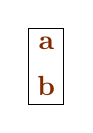
\begin{tikzpicture}

	\definecolor{odmlcolor}{rgb}{0.00,0.32,0.49}
	\definecolor{compcolor}{rgb}{0.51,0.16,0.00}
	
	\node(a1) [line width = 0pt,align=center,font=\bfseries, text=compcolor]{a};
	\node(b1)[below=0.1cm of a1,line width = 0pt,align=center,font=\bfseries, text=compcolor]{b};
	
	\begin{pgfonlayer}{background1}
		\draw [draw,fill=white] (a1.north east) rectangle (b1.south west);
	\end{pgfonlayer}

	
\end{tikzpicture}
}
\end{document}